\section{Analysis}
\label{sec:analysis}

\subsection{Mask overlap: a different circuit, not a reranking}
\label{sec:analysis-overlap}

Both \method{} and \baseline{} keep exactly 0.35\% of the 224
attn+MLP weight tensors---24.4M FP16 outliers each---yet they select largely
disjoint subsets. Against \baseline{} 2-bit (seed-matched), only 46\% of
\method{} outliers overlap ($J{=}0.298$); at 3-bit the overlap is 50\%
($J{=}0.331$). Thus ${\sim}54\%$ of \method{}'s FP16 budget protects weights
\baseline{} would quantize---this is not a minor reranking within the same
circuit (Figures~\ref{fig:jaccard-matrix}--\ref{fig:layer-module}).

\paragraph{Module-level divergence.}
MLP blocks contribute the largest \baseline{}-exclusive mass
(${\sim}2.9$--3.8M per projection), while \method{} retains more attention
weights (q/k/v\_proj exceed \baseline{}-only by ${\sim}0.4$--1.3M per head
type). Aggregated, \method{} adds 5.5M routing-centric outliers vs.\ 3.0M for
\baseline{}; \baseline{} adds 10.2M MLP-only vs.\ 7.7M. The circuit term
steers the budget toward mid-network routing while reshuffling which MLP
channels stay in FP16.

\paragraph{Layer-wise divergence.}
Disagreement peaks in mid layers 4--14 (layer 9 most divergent); early and
late layers agree more. The mid-stack is where task-specific schema and
compositional structure are processed in Llama-family models.

\paragraph{Seed sensitivity vs.\ method divergence.}
Cross-seed Jaccard among \method{} masks is 0.995--0.997 (only ${\sim}36$--56k
of 24.4M kept weights differ per seed pair), vs.\ 0.983--0.985 for \baseline{}
(${\sim}187$--214k). Cross-method $J{=}0.298$. Methods select different
circuits, not different seeds of the same circuit; \baseline{}'s polysemantic
CE gradients amplify calibration-shuffle effects more than the conjunction.

\begin{figure}[t]
\centering
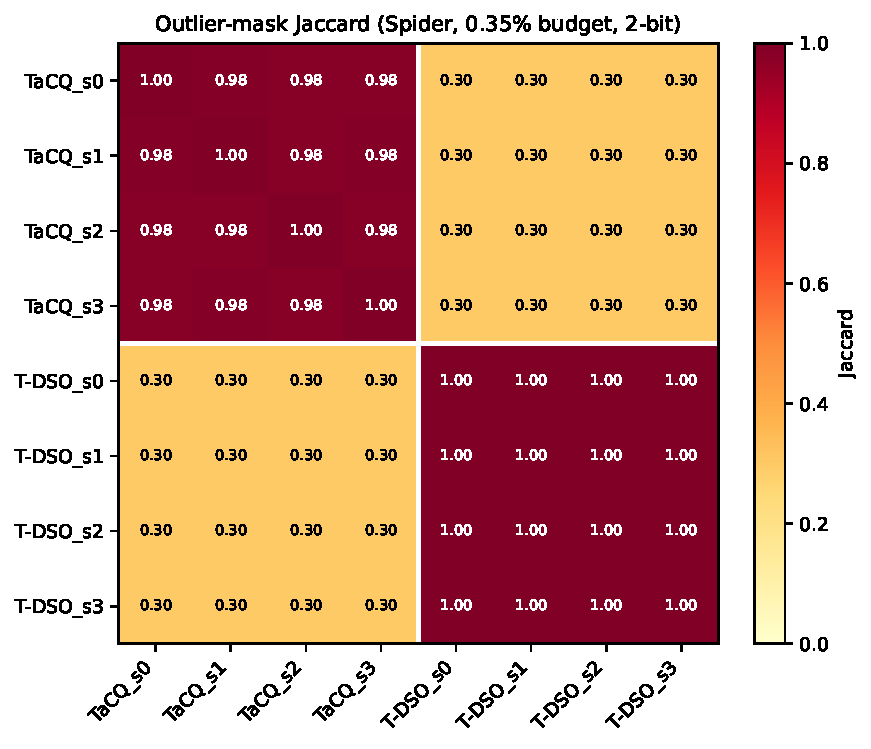
\includegraphics[width=0.7\linewidth]{figures/jaccard_matrix.pdf}
\caption{Cross-seed and cross-method Jaccard among 0.35\% outlier masks
(Spider, 2-bit). Diagonal blocks: within-method seeds ($J{>}0.98$);
off-diagonal: method gap ($J{\approx}0.30$).}
\label{fig:jaccard-matrix}
\end{figure}

\begin{figure}[t]
\centering
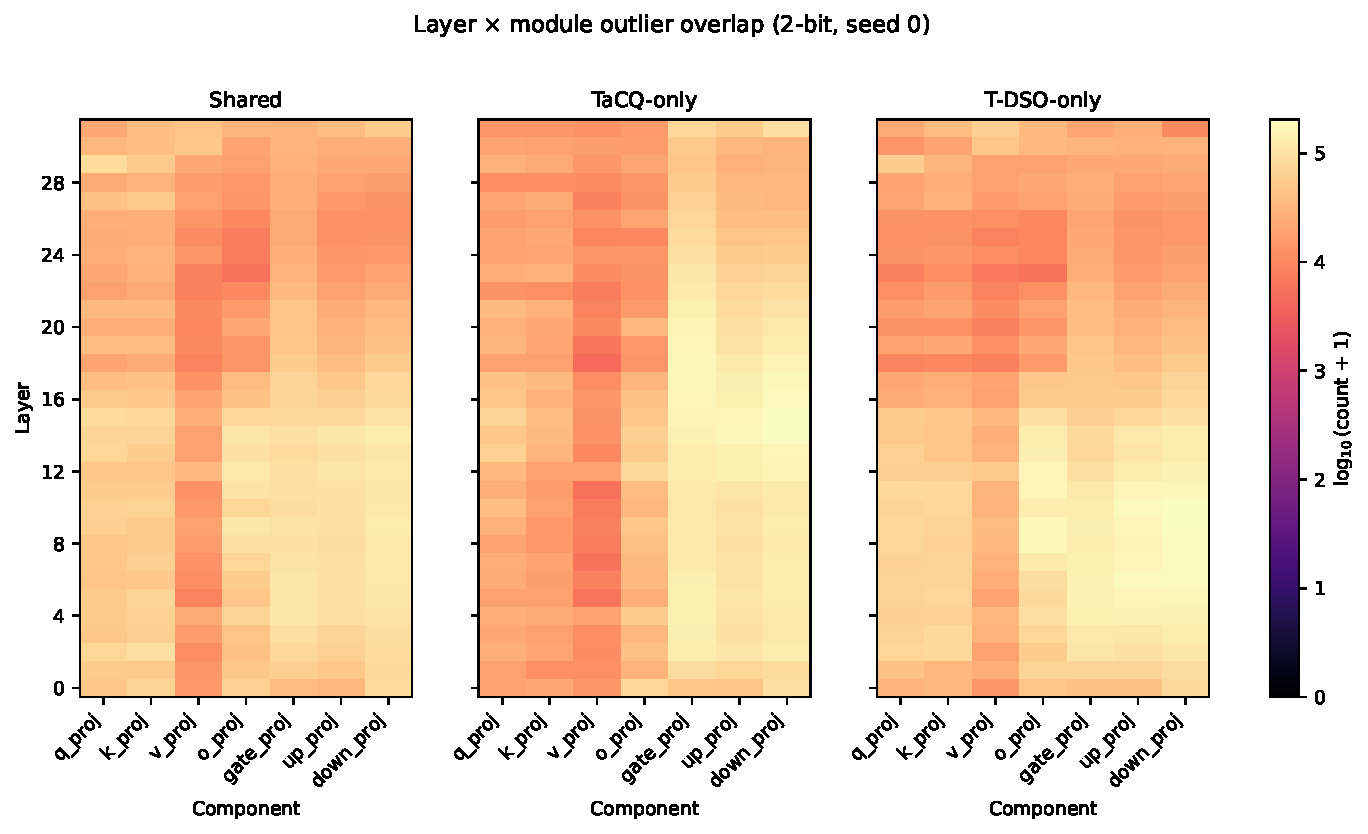
\includegraphics[width=0.9\linewidth]{figures/layer_module_heatmap.pdf}
\caption{Layer $\times$ module outlier decomposition (2-bit, seed 0): shared,
\baseline{}-only, and \method{}-only kept weights.}
\label{fig:layer-module}
\end{figure}

\subsection{Causal validation via targeted suppression}
\label{sec:analysis-knockout}

Scaling the 24.4M \method{}-masked weights by $\alpha{=}0.8$ on the FP16 model
(no quantization) drops Spider exec from 67.8\% to 38.9\% while short non-SQL
English probes remain fluent; the boost control ($\alpha{=}1.2$) also hurts
($-8.2$\,pt). The task-selective failure mode rules out the null that the mask
tags generic high-magnitude weights. A leak-free contrastive squeeze
($\alpha_{\text{task}}{=}1.05$, $\alpha_{\text{base}}{=}0.98$, selected on a
train holdout) yields $+1.0$\,pt dev exec over contemporaneous FP16.

\subsection{Why the native basis can beat the dictionary}
\label{sec:analysis-basis}

The MMLU-STEM reversal (mult$_{\text{free}}$ 44.2 vs.\ mult 38.9;
Table~\ref{tab:ablation}) suggests dictionary quality is task-dependent. Two
non-exclusive explanations: (i) \emph{coverage} --- CRV transcoders are trained
to reconstruct instruct-model MLP behavior on broad data; features that tile
mathematical CoT structure (GSM8K) may be better resolved than the
fine-grained factual retrieval MMLU stresses, so the transcoder's $\Delta a$
filter passes a noisier task set on MMLU; (ii) \emph{reconstruction error} ---
the alignment loss targets the transcoder's \emph{approximation} of the MLP
output; where reconstruction is weak, gradients partially chase approximation
artifacts. The native basis has zero reconstruction error by construction
(its decoder \emph{is} \texttt{down\_proj}), trading monosemanticity for
faithfulness. The conjunction with CE then filters its polysemantic noise.
This trade-off predicts the dictionary helps where its training distribution
matches the task and the native basis is safer elsewhere---a testable
criterion for future dictionary-aware PTQ.

\subsection{Efficiency and failure modes}
Saliency extraction matches \baseline{} asymptotics; the transcoder basis adds
per-layer encode/decode, the native basis adds only forward hooks. Union-style
combinations ($g_{\text{CE}}(1+\lambda g_{\text{align}})$) degenerate at 2-bit
(model rambles, no EOS), confirming that \emph{expanding} the CE mask with
circuit bonuses is worse than \emph{intersecting} the signals.
